\documentclass[11pt,a4paper]{article}

\usepackage[margin=25mm]{geometry}
\usepackage{amsmath,amssymb}
\usepackage{booktabs}
\usepackage{graphicx}
\usepackage{microtype}
\usepackage{xcolor}
\usepackage[hidelinks]{hyperref}

\graphicspath{{../figures/multi_interval/}}
\setlength{\parindent}{0pt}
\setlength{\parskip}{0.65em}
\newcommand{\Prob}{\mathbb{P}}
\title{Multi-Interval Evaluation Report\\\large All-On Model}
\author{}
\date{23 September 2026}

\begin{document}
\maketitle


\section{Two-interval allocation}


\begin{center}
\begin{tabular}{lll}
\toprule
Customer type & Assigned interval & Other interval\\
\midrule
Small & \(I_S\) & \(I_S\)\\
Medium & \(I_M\) & \(I_S\)\\
Large & \(I_L\) & \(I_S\)\\
\bottomrule
\end{tabular}
\end{center}

Let \(m_1\) and \(l_1\) be the numbers of medium and large customers assigned
to interval 1. The remaining \(n_M-m_1\) and \(n_L-l_1\) are assigned to
interval 2. Thus
\begin{align}
    A_1&=I_Mm_1+I_Ll_1+I_S(n_S+n_M-m_1+n_L-l_1),\\
    A_2&=I_M(n_M-m_1)+I_L(n_L-l_1)+I_S(n_S+m_1+l_1).
\end{align}

The model tries every integer allocation
\begin{equation}
    m_1\in\{0,\ldots,n_M\},\qquad l_1\in\{0,\ldots,n_L\},
\end{equation}
and chooses the allocation with the smallest maximum interval current:
\begin{equation}
    B^*(\boldsymbol n)=\min_{m_1,l_1}\max(A_1,A_2).
\end{equation}


A violation means \(A_1>T\) or \(A_2>T\). This is written as: 
\begin{equation}
    r_{\mathrm{two}}(\boldsymbol n)=
    \begin{cases}
        1,&B^*(\boldsymbol n)>T,\\
        0,&B^*(\boldsymbol n)\leq T.
    \end{cases}
\end{equation}



\section{Three-interval allocation}

Each medium or large customer is assigned to one of three intervals and
draws \(I_S\) in the other two. Small customers draw \(I_S\) in all three.
Let \(m_t,l_t\) be the medium and large counts assigned to interval \(t\).
Then
\begin{equation}
    m_1+m_2+m_3=n_M,\qquad l_1+l_2+l_3=n_L,
\end{equation}
where all counts are nonnegative integers. With
\(m_3=n_M-m_1-m_2\) and \(l_3=n_L-l_1-l_2\), the currents are
\begin{align}
    A_1&=I_Mm_1+I_Ll_1+I_S(n_S+m_2+m_3+l_2+l_3),\\
    A_2&=I_Mm_2+I_Ll_2+I_S(n_S+m_1+m_3+l_1+l_3),\\
    A_3&=I_Mm_3+I_Ll_3+I_S(n_S+m_1+m_2+l_1+l_2).
\end{align}
The optimal allocation minimizes the largest of the three currents:
\begin{equation}
    B_3^*(\boldsymbol n)=
    \min_{\substack{m_1+m_2+m_3=n_M\\l_1+l_2+l_3=n_L}}
    \max(A_1,A_2,A_3).
\end{equation}
A violation occurs if any interval exceeds \(T\), so
\begin{equation}
    r_{\mathrm{three}}(\boldsymbol n)=
    \begin{cases}
        1,&B_3^*(\boldsymbol n)>T,\\
        0,&B_3^*(\boldsymbol n)\leq T.
    \end{cases}
\end{equation}
The implementation computes the exact minimum by reusing solutions for
smaller remaining allocation problems. It does not use a heuristic or sampling.

\section{Optimal versus random allocation}

For \(K\in\{1,2,3\}\) intervals, random allocation means each medium and
large customer independently chooses one interval uniformly. We draw
\emph{one assignment per composition}, giving counts
\((m_1,\ldots,m_K)\) and \((l_1,\ldots,l_K)\), where
\begin{equation}
    \sum_{t=1}^K m_t=n_M,\qquad \sum_{t=1}^K l_t=n_L.
\end{equation}
For this realised assignment, calculate
\begin{equation}
    A_t^{\mathrm{random}}=I_Mm_t+I_Ll_t+I_S(N-m_t-l_t).
\end{equation}
The output is a binary violation outcome, not an average over assignments:
\begin{equation}
    v_{\mathrm{random},K}(\boldsymbol n)=
    \begin{cases}
        1,&\max_t A_t^{\mathrm{random}}>T,\\
        0,&\max_t A_t^{\mathrm{random}}\leq T.
    \end{cases}
\end{equation}


\section{Evaluation}

The calculation uses
\begin{equation}
    (I_S,I_M,I_L)=(20,40,100)\ \mathrm{A},\qquad
    N=40,\qquad T=1000\ \mathrm{A}.
\end{equation}


\begin{center}
\begin{tabular}{lr}
\toprule
Outcome & Compositions\\
\midrule
Already safe with one shared interval & 21\\
Made safe by two-interval allocation & 44\\
Still violating after optimal allocation & 796\\
\bottomrule
\end{tabular}
\end{center}

\begin{figure}[htbp]
    \centering
    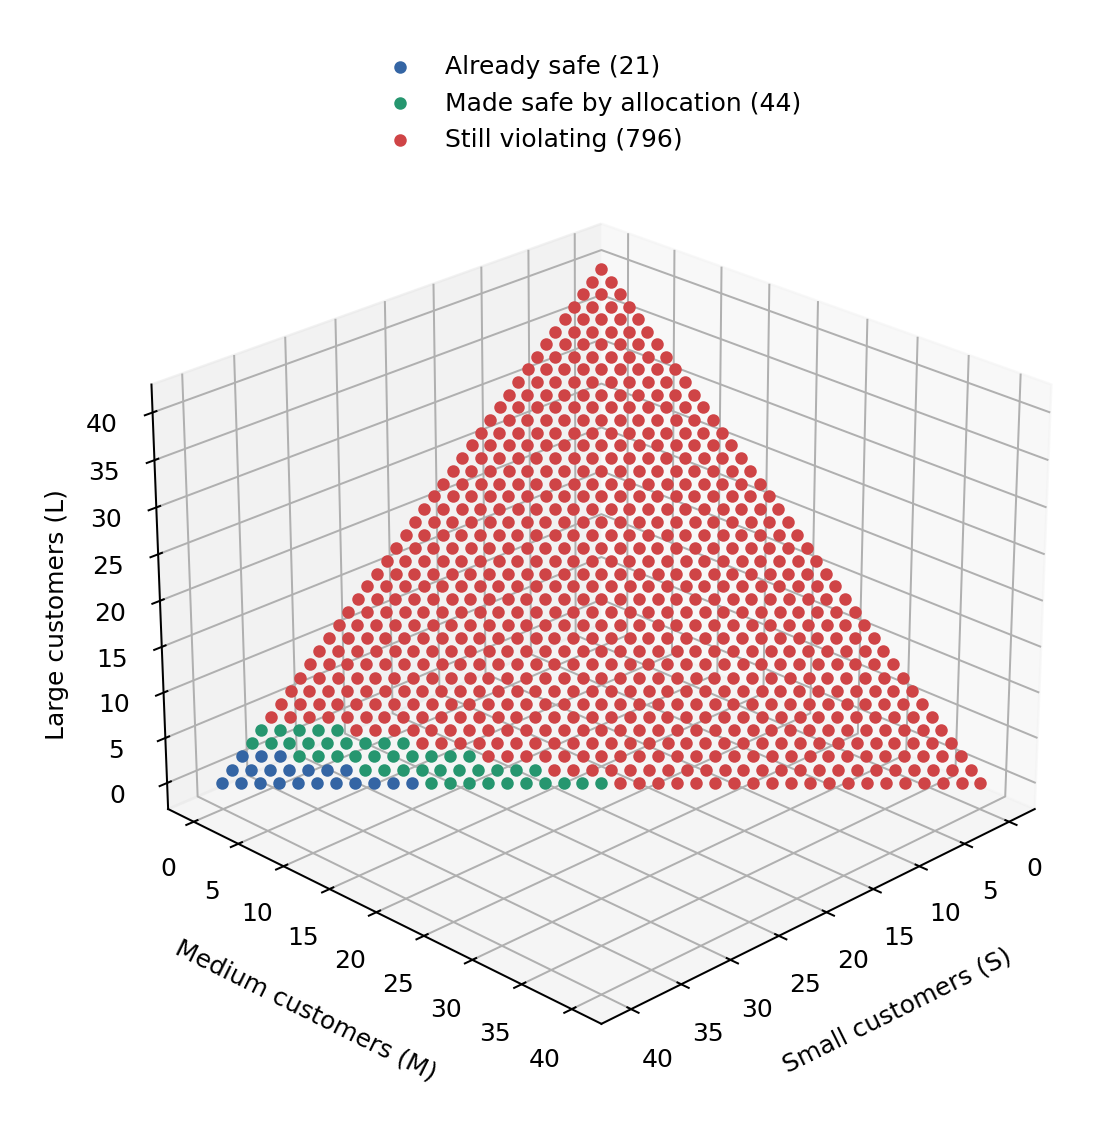
\includegraphics[width=0.82\textwidth]{allocation_3d.png}
    \caption{All-On two-interval allocation results. Colours show the
    outcome for each composition, not its trinomial probability.}
    \label{fig:allocation}
\end{figure}

\begin{center}
\begin{tabular}{lrr}
\toprule
Intervals & Optimal: points reversed & Random: points reversed\\
\midrule
1 & 0 & 0\\
2 & 44 & 24\\
3 & 112 & 48\\
\bottomrule
\end{tabular}
\end{center}


\begin{figure}[htbp]
    \centering
    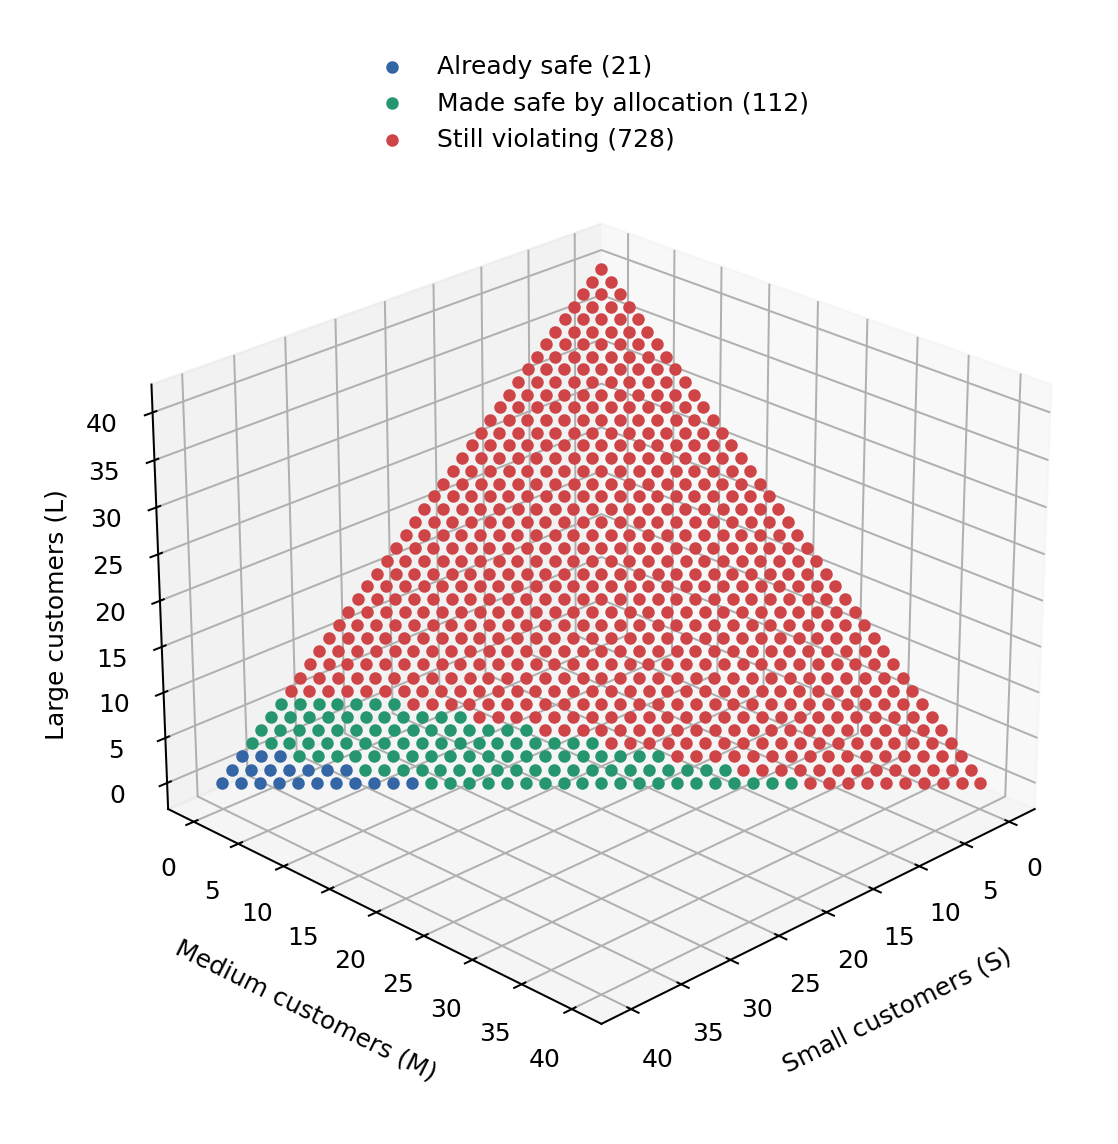
\includegraphics[width=0.82\textwidth]{allocation_3d_3_intervals.png}
    \caption{All-On three-interval optimal allocation results.}
    \label{fig:three-interval-allocation}
\end{figure}



\end{document}
